\documentclass[12pt,a4paper]{scrartcl}

\usepackage[a4paper, left=2cm, right=2cm, bottom=1cm, top=1cm, includeheadfoot]{geometry}
\usepackage[ngerman]{babel}
%\usepackage[utf8]{inputenc} % comment this if you uncomment utf8x
\usepackage[utf8x]{inputenc} % uncomment this if there are problems with 'ä', 'ü', 'ö'
\usepackage{ucs}
\usepackage[usenames,dvipsnames]{xcolor}
\usepackage[fleqn]{amsmath}
\usepackage{amsfonts}
\usepackage{amssymb}
\usepackage{color}
\usepackage{listings}
\usepackage{hyperref}
\usepackage{amsfonts}
\usepackage{scrpage2}
\usepackage{graphicx}
\usepackage{scrpage2} \pagestyle{scrheadings}
\usepackage[absolute]{textpos}
\usepackage{pdfpages}
\usepackage{alltt}
\usepackage{float}
\usepackage{array}
\usepackage{lastpage}
\usepackage{titling}

% command to format a collum in a table centered
\newcolumntype{C}[1]{>{\centering\arraybackslash}m{#1}}

\definecolor{mygray}{rgb}{0.95,0.95,0.95}
\lstset{language=[Visual]Basic, morekeywords={param, local}}

\lstset{
   literate={ö}{{\"o}}1
           {ä}{{\"a}}1
           {ü}{{\"u}}1
           {ß}{{\ss}}1
           {é}{{\'e}}1,
   inputencoding=ansinew,
   extendedchars=true,
   basicstyle=\scriptsize\ttfamily,
   numberstyle=\scriptsize,
   breaklines=true,
   tabsize=2,
   numbersep=5pt
}

\lstdefinestyle{ccode}{
   language=C,
   keywordstyle=\color{blue}\bfseries,
   stringstyle=\color{BrickRed}\ttfamily,
   commentstyle=\color{OliveGreen}\ttfamily,
   showspaces=false,
   showstringspaces=false,
   showtabs=false,
   numbers=left,
   frame=single
}
\lstdefinestyle{cplusplus}{
   language=C++,
   keywordstyle=\color{blue}\bfseries,
   stringstyle=\color{BrickRed}\ttfamily,
   commentstyle=\color{OliveGreen}\ttfamily,
   showspaces=false,
   showstringspaces=false,
   showtabs=false,
   numbers=left,
   frame=single
}
\lstdefinestyle{csharp}{
   language=[sharp]c,
   keywordstyle=\color{blue}\bfseries,
   stringstyle=\color{BrickRed}\ttfamily,
   commentstyle=\color{OliveGreen}\ttfamily,
   showspaces=false,
   showstringspaces=false,
   showtabs=false,
   numbers=none,
   frame=single
}
\lstdefinestyle{vhdlcode}{
   language=VHDL,
   keywordstyle=\color{blue}\bfseries,
   stringstyle=\color{BrickRed}\ttfamily,
   commentstyle=\color{OliveGreen}\ttfamily,
   showspaces=false,
   showstringspaces=false,
   showtabs=false,
   numbers=left,
   frame=single
}
\lstdefinestyle{customoutput}{
   backgroundcolor=\color{mygray},
   numbers=none,
   showspaces=false,
   showtabs=false
}

\newcommand{\includeccode}[1]{\lstinputlisting[style=ccode]{#1}}
\newcommand{\includecpluspluscode}[1]{\lstinputlisting[style=cplusplus]{#1}}
\newcommand{\includecsharpcode}[1]{\lstinputlisting[style=csharp]{#1}}
\newcommand{\includevhdlcode}[1]{\lstinputlisting[style=vhdlcode]{#1}}
\newcommand{\includetextfile}[1]{\lstinputlisting[style=customoutput]{#1}}

%pictures
\newcommand{\includepicture}[4]{
\begin{figure}[H]
\centering
\includegraphics[scale=#2]{#1}
\caption{\textit{#4}}
\label{fig:#3}
\end{figure}
}

%~~~~~~~~~~~~~~~~~~~~~~~~~~~~~~~~~~~~~~~~~~~~
% Some constants for header, footer and tile page
%~~~~~~~~~~~~~~~~~~~~~~~~~~~~~~~~~~~~~~~~~~~~

% Format der Kopf-und Fußzeile
\pagestyle{scrheadings}
\clearscrheadfoot

\ihead{\emph{FH Hagenberg / ESD}}
\chead{\emph{On Chip Signal Processing}}
\ohead{\emph{RTL Implementierung RX}}

\ofoot{\emph{\thepage \ / \ \pageref{LastPage}}}

\begin{document}  % Beginn des Textes

\pretitle{%
  \begin{center}
  \LARGE
  
\includegraphics[scale=0.1]{../img/logo}\\[\bigskipamount]
}
\posttitle{\end{center}}

\title{On Chip Signal Processing - RTL Implementierung RX}
\subtitle{Sommersemester 2018}
\author{Daniel Ferrari \\ Nikolaus Haminger \\ Florian Kitzer \\ Matthäus Kücher \\ Alexander Traxler}

% Insert name and etc. into pdf
%\begin{textblock*}{60mm}(45mm,58mm)
%\firstname \ \lastname , \sfirstname \ \slastname
%\end{textblock*}

\maketitle % Titelseite erstellen
%\includepdf[pages=-]{../spv_ue05.pdf}
\tableofcontents

\newpage

\section{Übersicht}
\subsection{Spezifikation}
In diesem Projekt sollte eine OFDM-RX-Architektur in VHDL implementiert werden. Ein grobes Blockdiagramm dieser RX-Komponente war vorgegeben und ist in Abbildung \ref{fig:big_picture} sichtbar.

\includepicture{../img/big_picture.png}{0.45}{big_picture}{Blockschaltbild der gesamten RX-Kette.}

\subsection{Implementierung}
Die Implementierung wurde weitgehend nach dem Vorbild des spezifizierten Blockschaltbildes vollzogen. Allerdings wird der Offset und das Delay in der Entity \emph{Coarse Alignment} gehandhabt, weshalb die Leitungen \texttt{rx\_data\_delay}, \texttt{rx\_data\_offset} und \texttt{interp\_mode} zwischen \emph{Interpolation} und \emph{Coarse Alignment} eliminiert wurden.

\subsection{Toplevel-Simulation}
Zur Verifikation der gesamten RX-Kette wurde eine Toplevel-Simulation erstellt. Für den Vergleich der Ergebnisse der Hardware-Kette wurde ein Golden Model in Python implementiert. Diese Implementierung berechnet die Input-Signale für die Hardware-Simulation (\texttt{rx\_data\_i}), speichert diese in CSV-Dateien ab und simuliert die gesamte RX-Kette in einer Hardware-ähnlichen Implementierung. Die Ergebnisse des Golden Models werden ebenfalls abgespeichert und am Ende der Hardware-Simulation mit eben jenen Ergebnissen verglichen. Außerdem werden \emph{BER} und \emph{EVM} berechnet sowie Konstellationdiagramme jeweils für beide Simulationen erstellt.

\vspace{10pt}
\noindent
\textbf{Achtung}: Matlab wird nicht benötigt, da das gesamte Golden Model sowie die Verifikation in Python implementiert wurde (mit Fixed-Point-Repräsentation und Taylor-Approximation der Interpolation). Die Gründe für diese Maßnahme sind die bessere Performance von Python, die einfachere Interaktion aus der Modelsim-Simulation und die bessere Strukturierungsmöglichkeit des Codes.

\subsubsection{Anleitung zur Toplevel-Simulation}
Eine ausführliche Anleitung befinden sich in der \texttt{README.md} des Repositories. Hier kurz noch einmal zusammengefasst:

\vspace{5pt}
\noindent
\textbf{Anforderungen}:
\begin{itemize}
\item Modelsim oder Questasim
\item Python3 (https://www.python.org/downloads/)
\item numpy und matplotlib (\texttt{pip install numpy matplotlib})
\end{itemize}

\vspace{5pt}
\noindent
\textbf{Ausführung}:\\
Um die Simulation zu starten, einfach \texttt{start\_rx\_simulation.bat <cmd|gui|clean>} oder\\ \texttt{start\_rx\_simulation.sh <cmd|gui|clean>} im Root-Folder des Repositories ausführen.

\subsubsection{Simulations-Output}
Nachfolgend ist der Output einer Simulation von 3 unterschiedlichen RX-Sequenzen zu sehen.
\includetextfile{sim_output.txt}

\subsubsection{Konstellationsdiagramm}
Abbildung \ref{fig:plot0} zeigt die Konstellationsdiagramme einer Symbol-Sequenz für die Golden-Model- und die Hardware-Simulation. Die Plots sind nach einer Simulation im Ordner\\ \texttt{src/grpRx/unitTopLevel/sim} zu finden.
\includepicture{../img/scatter_plot0.png}{0.55}{plot0}{Konstellationsdiagramme der Golden-Model- und Hardware-Simulationen}

\subsubsection{Synthese}
Für das implementierte Gesamtsystem wurde eine Synthese mit \texttt{Quartus} durchgeführt. Als Zielplattform wurde der FPGA 5CSXFC6D6F31C6 des DE-10 Standard-Boards verwendet. Folgende Ressourcen werden für das Gesamtsystem benötigt bei einer Symbollänge von 320 Samples und einer Überabtastung von 16.
Diese sind in der nachstehenden Tabelle \ref{tab:resources_coarse} zu sehen.

\begin{table}[H]
\centering
\begin{tabular}{|c|c|}
\hline
\textbf{Ressource} & \textbf{Menge} \\ \hline
Register & 15,652 \\ \hline
ALMs & 7,920 / 41,910 \\ \hline
M10K-Blöcke & 42 / 553 \\ \hline
Block Memory Bits & 134,896 / 5,662,720 \\ \hline
Total Block Memory Implementation Bits & 430,080 / 5,662,720 \\ \hline
DSP-Blöcke & 11 / 112 \\ \hline
Pins (theoretisch) & 48 / 499 \\ \hline
\end{tabular}
\caption{Tabelle mit benötigten Ressourcen.}
\label{tab:resources_coarse}
\end{table}

Die Timing-Analyse hat ergeben, dass das Gesamtsystem im 1100mV-85C-Model mit einer maximalen Taktfrequenz von 105,34 MHz betrieben werden kann. Als Systemtakt sind 100 MHz vorgesehen.

\section{Komponenten}

\subsection{Interpolation}
Die Aufgabe des Blockes \texttt{Interpolation} ist das Upsampling der einzelnen Symbole um 2\textsuperscript{n} Symbole. Als Interpolationsalgorithmus wird die Taylor-Reihe verwendet mit
\\
\\

$ f(x)=f(x\textsubscript{0}	) +f\textsuperscript{'} (x\textsubscript{0}) (x-x\textsubscript{0})+\frac{f\textsuperscript{''}(x\textsubscript{0})}{2!}(x-x\textsubscript{0})\textsuperscript{2} $,
\\
\\

\noindent wobei die erste und zweite Ableitung aus den ursprünglichen Samples berechnet wird



\subsubsection{Architektur}
Für die Berechnung der Interpolationssymbole durch die Taylor-Reihe werden jeweils 3 Symbole benötigt. Zu Begin wird deshalb so lange gewartet, bis 3 Symbole gespeichert werden. Danach kann nun die erste und zweite Abbleitung durch
\\
\\
$f\textsuperscript{'}(x\textsubscript{0})=f(x\textsubscript{1})-f(x\textsubscript{0}) $\\
\noindent $f\textsuperscript{''}(x\textsubscript{0})=f(x\textsubscript{2})-2f(x\textsubscript{1})+f(x\textsubscript{0}) $
\\
\\
\noindent berechnet werden und somit mit jedem Takt ein neues interpoliertes Symbol ausgegeben werden. Wie viele Symbole interpoliert werden sollten, wird als generic Parameter mitgegeben.

\includepicture{../img/arch_interpolation}{0.65}{arch_interpolation}{Architektur von \texttt{Interpolation}}.



\subsubsection{Simulation}

Für die korrekte Funktionalität des Interpolationsblockes wurde Matlab und Modelsim für die Simulation verwendet. Dazu wurden zufällige Symbole in Matlab generiert. Diese Symbole wurden einmal mit der Matlab Funktion und einmal mit vhdl interpoliert, geplotet und verglichen.


\includepicture{../img/interpolation_test.png}{0.62}{interpolation_test}{Testausgabe von \texttt{Interpolation}}.
\includepicture{../img/interpolation_wave.png}{0.35}{interpolation_wave}{Waveausgabe von \texttt{Interpolation}}.

\noindent In Abbildung \ref{fig:interpolation_wave} ist die Waveform der Simulation zu sehen. Es ist zu erkennen, dass das Upsampling erst beim Empfangen des dritten Symboles startet und danach jeden Takt ein Upsample-Symbol berechnet.

\subsubsection{Synthese}
\includepicture{../img/synthese_interp.png}{1}{Synthese_Interplation}{Syntheseergebnis von \texttt{Interpolation}}.

Abbildung \ref{fig:Synthese_Interplation} zeigt den Ressourcenverbrauch für den Interpolationsblock.
Die Timing-Analyse hat ergeben, dass die \texttt{Interpolation} im 1100mV-85C-Model mit einer maximalen Taktfrequenz von 107,12 MHz betrieben werden kann. Als Systemtakt sind 100 MHz vorgesehen.

\subsection{Coarse Alignment}
Die Aufgabe des \texttt{Coarse Alignment} ist das Finden des Beginns einer OFDM-Übertragung. Für das Finden der Beginns wird die Methode nach Schmidl und Cox verwendet. Dazu wird in Hardware die Korrelation über zwei identische Halbsymbole (= Trainingssymbol) berechnet und das Maximum detektiert. Danach werden fortlaufend die Steuersignale \texttt{start\_of\_symbol} und \texttt{data\_valid} des Datenstromes gesetzt und nach den Vorgaben des \texttt{Fine Alignment} korrigiert.

\subsubsection{Architektur}

In Abbildung \ref{fig:arch_coarse} ist ein grober Überblick über die Implementierung gegeben. Die Implementierung beginnt links oben mit dem Eintreffen der I- und Q-Komponente des Empfangssignals. Beide Komponenten haben Datenbreite von 12 Bit signed. Die eintreffenden Daten werden in einem Ringbuffer mit der halben Symbollänge gespeichert, wodurch die Daten um die halbe Symboldauer verzögert werden. Die darauffolgenden Multiplizierer und Addierer stellen die komplexe Multiplikation der Korrelationsberechnung dar.

\begin{center}
\includepicture{../img/arch_coarse_alignment.png}{0.65}{arch_coarse}{Architektur des \texttt{Coarse Alignment}. Links oben sind die Eingangsdaten als I und Q Anteil zu sehen. Darauf folgt die Korrelationsberechnung, gefolgt von der FSM zum Erkennen des Maximums. Unten im Bild ist die Logik zur Steuersignalgenerierung zu sehen.}
\end{center}

Die Ergebnisse der komplexen Multiplikation werden in Register gespeichert, bevor diese im Zielregister aufsummiert werden. Nach der komplexen Multiplikation haben sowohl I- als auch Q-Komponente eine Datenbreite von 25 Bit signed. Auch die Ergebnisse der komplexen Multiplikation werden in einem Ringbuffer abgelegt, damit diese nach der halben Symboldauer wieder subtrahiert werden können. Dadurch entsteht der Effekt eines gleitenden Korrelationsfensters über dem Empfangssignal. Für das Ergebnis der Korrelation wird eine Datenbreite von 35 Bit signed verwendet. \vspace{0.5 cm}

Das berechnete Korrelationssignal wird einer FSM zugeführt. Diese FSM beginnt ein Maximum auf dem Korrelationssignal zu suchen, wenn dieses einen gegebenen Schwellwert über-schreitet. Ein Maximum wurde dann gefunden, wenn der aktuelle Signalwert im Vergleich zum vorhergehenden Signalwert beginnt zu sinken. Ab diesen Zeitpunkt werden die Daten vom \texttt{Coarse Alignment} vom Eingang zum Ausgang weitergegeben. Für die Auswertung wird nur die I-Komponente des Korrelationssignals verwendet, da diese das Maximum ausbildet. Die FSM steuert danach die Delay-Logik, die für die Generierung der Steuersignale \texttt{start\_of\_symbol} und \texttt{data\_valid} zuständig ist. Diese besteht intern aus zwei Zählern. Der erste Zähler ist für die Generierung des \texttt{data\_valid}-Signals zuständig. Wenn dieser Zähler einen Überlauf hat, wird das Signal für eine Taktperiode auf 1 gesetzt und der zweite Zähler ebenfalls erhöht. Hat der zweite Zähler einen Überlauf wird das \texttt{start\_of\_symbol}-Signal für eine Taktperiode auf 1 gesetzt. Die Korrektur des Delays wird über die \texttt{inc}- und \texttt{dec}-Leitungen durch das \texttt{Fine Alignment} gesteuert. Ist eine der beiden Leitungen 1 wird der erste Zähler der Delay-Logik entsprechend korrigiert, wodurch die Steuersignale um ein Datum nach vorne oder nach hinten verschoben werden. Die Auswertung der Leitungen wird immer zu Beginn eines neuen OFDM-Symbols durchgeführt.

\subsubsection{Simulation}
Für die Simulation wurde sowohl Matlab als auch Modelsim verwendet. Mit Hilfe von Matlab wurde ein Empfangssignal mit der Länge von 100 Symbolen generiert. In diesem Empfangssignal ist das Trainingssymbol an der dritten Stelle. Der Beginn der Korrelation des generierten Empfangssignals ist in Abbildung \ref{fig:signal_coarse} zu sehen. Der grün umrandete Signalteil stellt das Trainingssymbol dar. Das obere Diagramm zeigt das Ergebnis der iterativen Implementierung. Das untere Diagramm zeigt das Ergebnis der formalen Implementierung. Es ist zu erkennen, dass beide Diagramme bis auf eine Verschiebung den gleichen Kurvenverlauf darstellen.

\begin{center}
\includepicture{../img/p_signal.png}{0.33}{signal_coarse}{Beginn des Empfangssignals. Oben ist die iterative und unten die formale Implementierung dargestellt. Der grün umrandete Signalteil stellt das Trainingssymbol dar.}
\end{center}

Für die Simulation wurde der Simulator \texttt{Modelsim} verwendet. Als Testframework wurde UVVM verwendet. Dadurch war es möglich ein besser strukturierte VHDL-Testbench zu entwerfen. In der Simulation wird das mit Matlab generierte Empfangssignal an den \texttt{Coarse Alignment}-Block angelegt und auf die Detektion des Trainingssymbols gewartet. Nach der Detektion wird das Timing der Steuersignale überprüft. Darauf wird überprüft, ob die Daten korrekt vom Block weiter gegeben werden. Am Ende wird das Verhalten im Zusammenhang mit den Steuerleitungen vom \texttt{Fine Alignment} und dem \texttt{init}-Signal überprüft. In Abbildung \ref{fig:sim_coarse} ist ein Teil der Waveform der Simulation zu sehen. Die berechnete Korrelation in der Simulation stimmt mit der Berechnung in Matlab überein.

\begin{center}
\includepicture{../img/sim_coarse.png}{0.30}{sim_coarse}{Waveform der Simulation des \texttt{Coarse Alignment}. Im unteren Teil der Bildes ist die Korrelation des Empfangssignales zu erkennen.}
\end{center}

Um die Simulation starten zu können, müssen die Skripen \texttt{compile\_uvvm.do}, \texttt{compile.do} und \texttt{run\_simulation.do} in dieser Reihenfolge ausgeführt werden.

\subsubsection{Synthese}
Für das implementierte \texttt{Coarse Alignment} wurde eine Synthese mit \texttt{Quartus} durchgeführt. Als Zielplattform wurde der FPGA 5CSXFC6D6F31C6 des DE-10 Standard-Boards verwendet. Folgende Ressourcen werden für das \texttt{Coarse Alignment} benötigt bei einer Symbollänge von 320 Samples und einer Überabtastung von 16.
Diese sind in der nachstehenden Tabelle \ref{tab:resources_coarse} zu sehen.

\begin{table}[H]
\centering
\begin{tabular}{|c|c|}
\hline
\textbf{Ressource} & \textbf{Menge} \\ \hline
Register & 232 \\ \hline
ALMs & 182 / 41,910 \\ \hline
M10K-Blöcke & 12 / 553 \\ \hline
Block Memory Bits & 122,880 / 5,662,720 \\ \hline
Total Block Memory Implementation Bits & 245,760 / 5,662,720 \\ \hline
DSP-Blöcke & 2 / 112 \\ \hline
Pins (theoretisch) & 72 / 499 \\ \hline
\end{tabular}
\caption{Tabelle mit benötigten Ressourcen.}
\label{tab:resources_coarse}
\end{table}

Die Timing-Analyse hat ergeben, dass das \texttt{Coarse Alignment} im 1100mV-85C-Model mit einer maximalen Taktfrequenz von 111,68 MHz betrieben werden kann. Als Systemtakt sind 100 MHz vorgesehen.

\subsection{Cyclic Prefix Removal}

\subsection{FFT Wrapper}
Für den FFT-Block  wurde ein Wrapper für die Altera-FFT implementierung gebaut. Dazu werden 256 I/Q Symbole in einem Buffer gespeichert. Dieser Buffer wird der Altera FFT implemssentierung übergeben, die Steuersignale Start und Valid gesetzt und die Berechnung der Altera FFT beginnt. Wenn die Altera FFT-Implementierung die Berechnung fertig hat, werden die Steuerung des Ausganges Valid und StartOfPacket gesetzt. Somit kann das FFT-Ergebnis wieder in den internen Buffer gespeichert werden. Die unbenutzen Frequenzen werden herausgefiltert und die Daten an das FineAlignment weitergegeben.

\includepicture{../img/arch_fft.png}{0.65}{arch_fft}{Architektur von \texttt{FFT Wrapper}}.

\subsubsection{Simulation}
Um das Ergebnis zu evaluieren, wurden OFDM Symbole in Matlab mithilfe der Altera-IFFT generiert. Diese Symbole wurden der VHDL Beschreibung übergeben und das Ergebnis mit den ursprünglichen Symbolen verglichen. Würde es bei der FFT zu Problemen kommen, werden Error Signale als Ausgang der FFT-Altera gesetzt, welche bei den Tests überprüft wurden.

\subsection{Fine Alignment}

Das \texttt{Fine Alignment} kümmert sich um die Feinjustierung der Symbole über die Phase. Eine Phasenverschiebung im Frequenzbereich ist gleichbedeutend mit einer zeitlichen Verschiebung im Zeitbereich. Nach der groben Korrektur (Coarse Alignment) besteht immer noch ein Phasenfehler, der über mehrere Symbole hinweg korrigiert werden kann.\\
\\


\subsubsection{Architektur}
Das Blockdiagramm in \autoref{fig:FineAlignmentBlock} verdeutlicht den Aufbau des Fine Alignment. Zur Berechnung des Phasenfehlers werden, aufgrund der Linearphasigkeit des Filters in diesem Bereich, nur die ersten 32 Symbole verwendet. Die Symbole werden zu Beginn in den 1. Quadranten (First Quadrant) gebracht. Die Inphase- und Quadratur-Komponenten werden separat aufsummiert. Der Phasenfehler ergibt sich durch die Subtraktion der Inphase- von der Quadratur-Komponente (Q-I). Anders ausgedrückt Imaginärteil - Realteil. Dieser Ansatz ist möglich, da wir QPSK verwenden, wo nur ein Symbol pro Quadrant vorhanden ist. Ergibt die Subtraktion 0 so ist kein Phasenfehler gegeben. Andernfalls ist nur das Vorzeichen interessant, welches die Richtung für die Verschiebung im Zeitbereich angibt.\\
\\
Hat ein komplettes Symbol das Fine Alignment durchlaufen, erwartet sich das Coarse Alignment eine Entscheidung ob \textit{increment} oder \textit{decrement}. Keines von beiden ist in der Implementierung nicht möglich. Die inc und dec Leitungen sind direkt verknüpft mit dem Vorzeichen des Ergebnisse der Phasenberechnung. Das Ergebnis schwankt somit bei der Berechnung (innerhalb der 32 Symbole) stark und ist danach fix auf einem Wert für den Rest des Symbols (bis zum Start des nächsten). Dadurch schwankt das Fine Alignment immer zwischen dem besten und zweitbesten Wert für Korrektur der Phase. Wichtig für die Implementierung sind die Bitbreiten für die Summen von Imaginär- und Realteil (Reg Imaginär, Reg Real). Diese berechnen sich aus 32 * 12 Bit = 17 Bit.

\begin{figure}[htbp] 
	\centering
	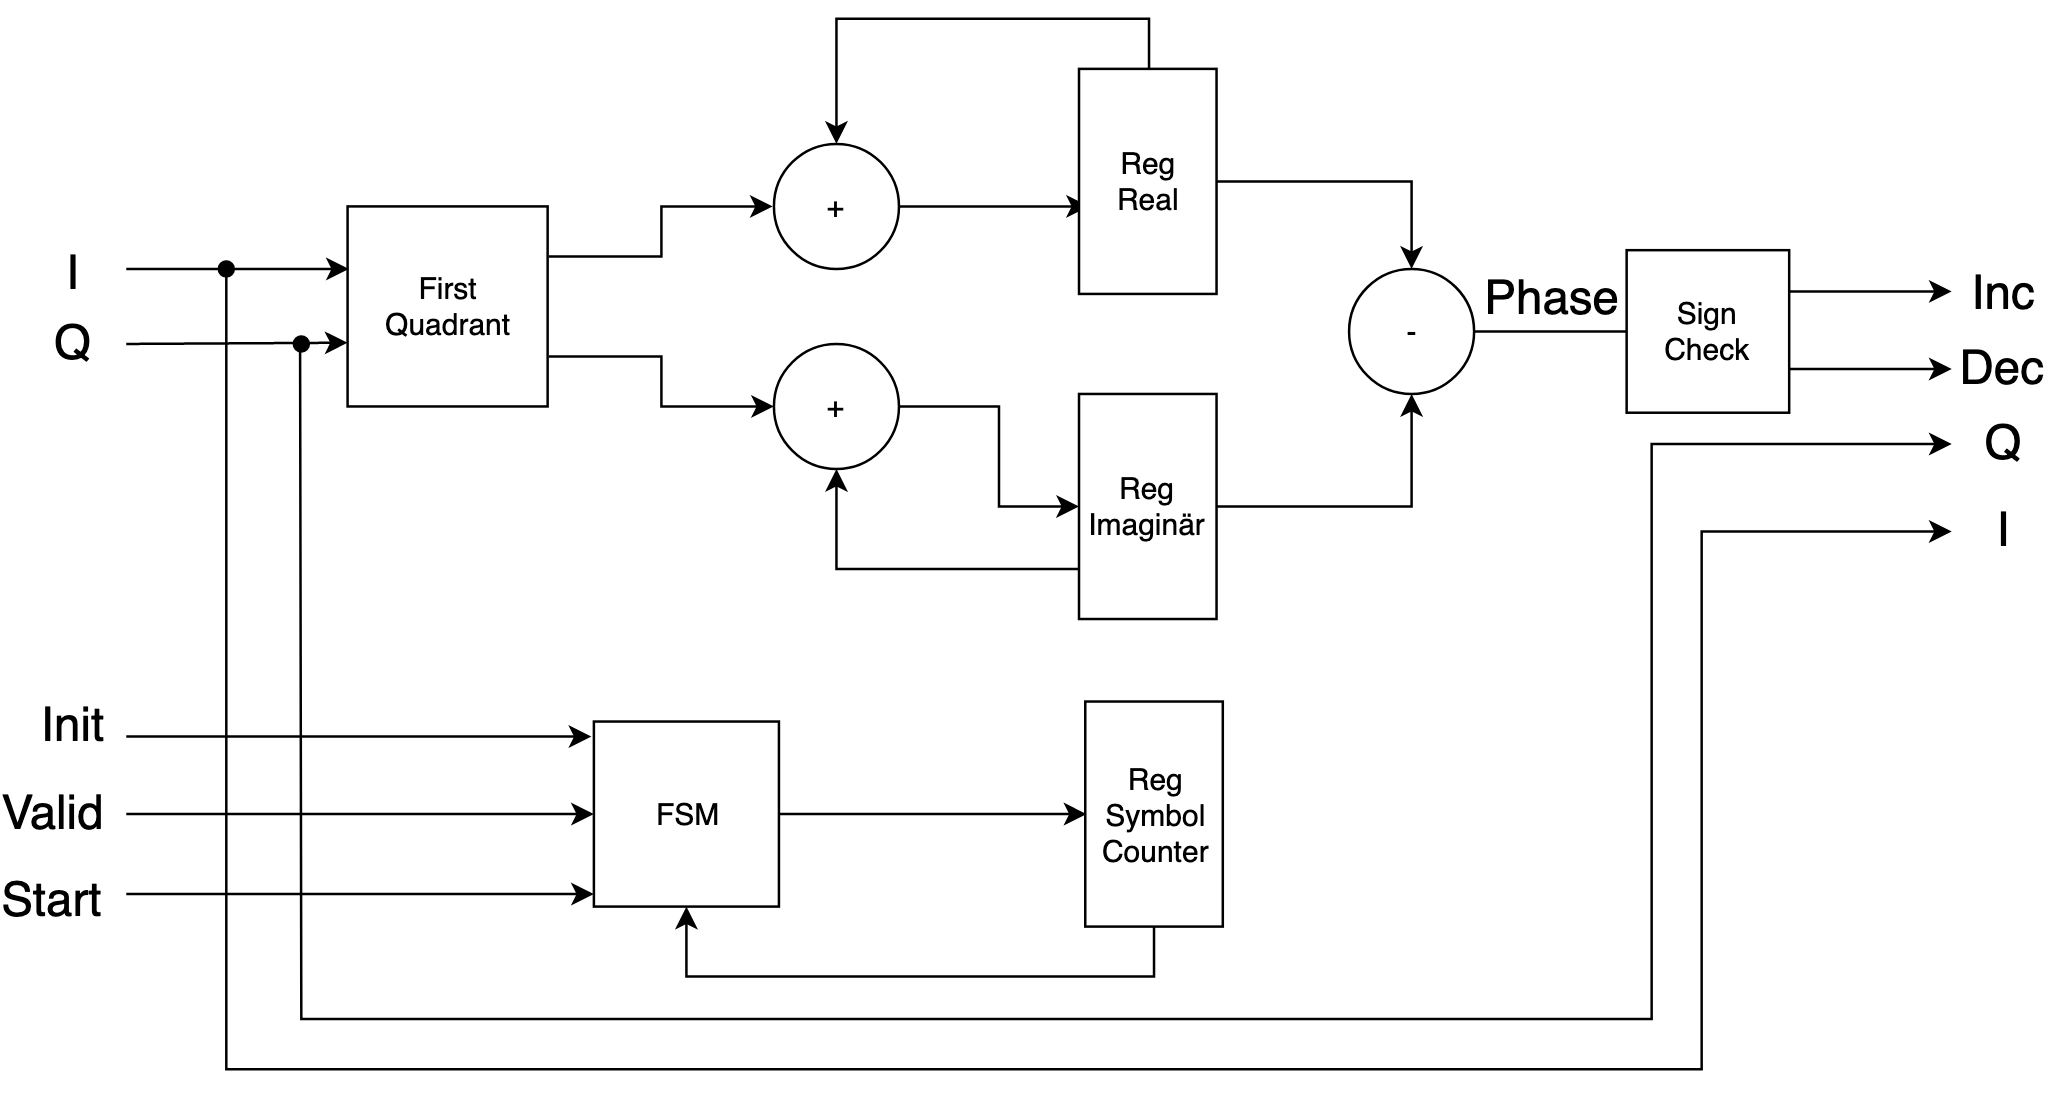
\includegraphics[width=0.9\textwidth]{../img/FineAlignmentBlock.png}
	\caption{Blockdiagramm des Fine Alignment}
	\label{fig:FineAlignmentBlock}
\end{figure}

\subsubsection{Simulation}
Getestet wurde mit UVVM. Die Testbench vom Coarse Alignment wurde wiederverwendet und adaptiert für das Fine Alignment. Geprüft werden Reset-Condition, Ergebnis von inc und dec nach den ersten 32 Werten des Symbols und die Init-Condition nach dem Symbol. Aufgrund der Implementierung ist im Reset und im Init die dec Leitung aktiv und die inc Leitung inaktiv. Die Leitungen werden aber erst beim Übergang von Init auf Phase in diesen Zustand versetzt. Ansonsten würde das eigentliche Ergebnis nach den 32 Symbolen verloren gehen (vgl. \autoref{fig:FineAlignmentSim}).\\
\\
Um Werte für die Simulation zu generieren wurde ein Matlab-Modell des Fine Alignment erstellt. In jedem Schritt wo korrigiert wird können die Daten aus dem Skript für die Simulation gespeichert werden. Lediglich die Vergleiche in der Testbench der inc und dec Leitungen müssen entsprechend angepasst werden.

\begin{figure}[htbp] 
	\centering
	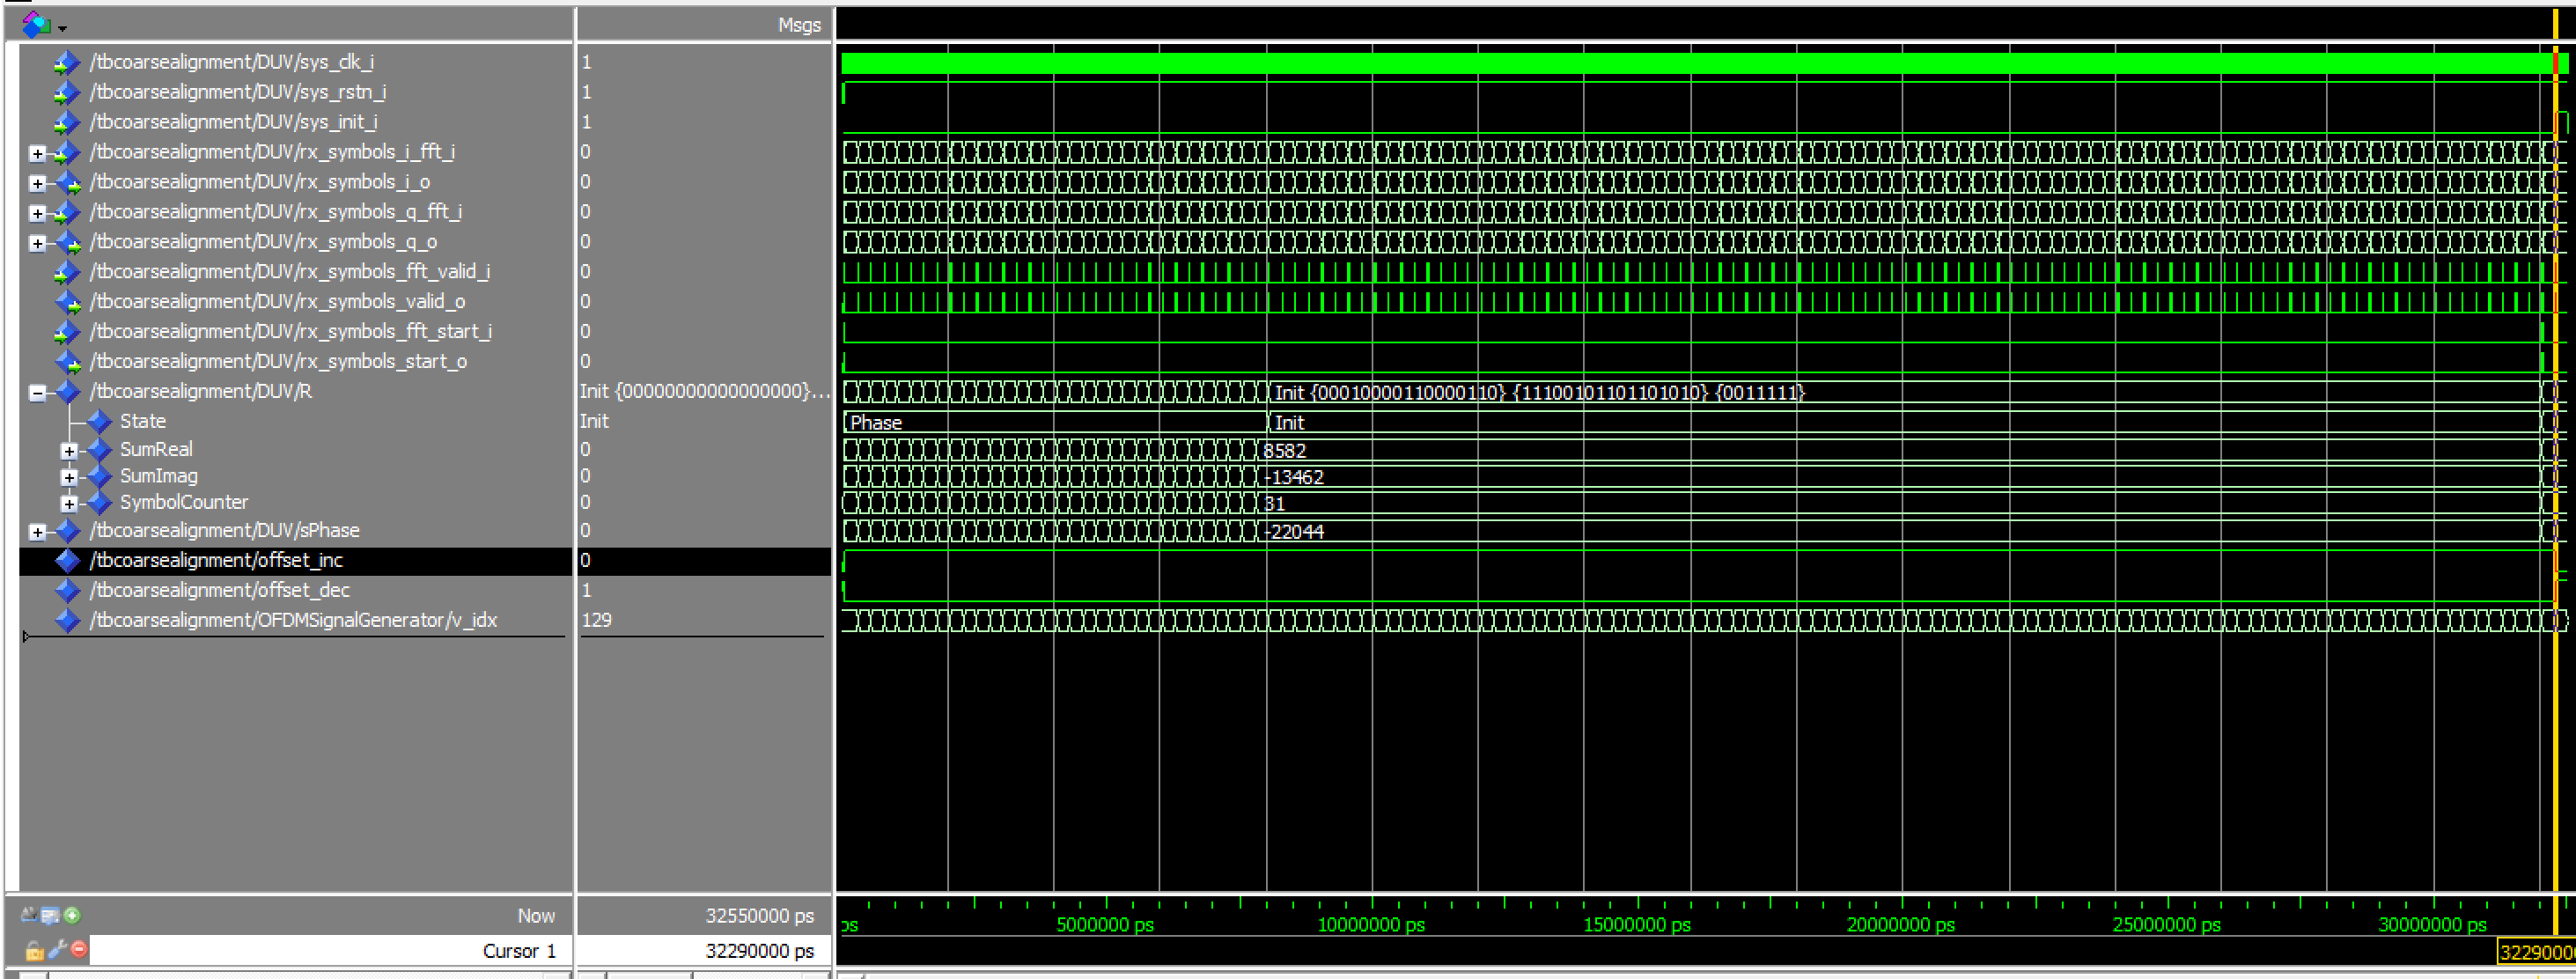
\includegraphics[width=0.9\textwidth]{../img/FineAlignmentSim.png}
	\caption{Simualtion mit Init-/Reset-Zustand beim Cursor.}
	\label{fig:FineAlignmentSim}
\end{figure}

\subsubsection{Synthese}
Die Synthese wurde ebenfalls für den Device 5CSXFC6D6F31C6 durchgeführt. Eingestellt bei den generics wurden eine Symbollänge von 128 und eine Bitbreite von 12 Bit. Die Implementierung könnte für die Synthese noch verbessert werden. Die größer/kleiner Vergleiche für die Quadranten können auf ein gleich abgeändert werden, wenn man auf die Vorzeichen prüft. Register können ebenfalls beim \textit{SymbolCounter} gespart werden, wenn man ihn auf die 32 Symbole beschränkt. Diese Optimierungen wurden nicht mehr durchgeführt. \autoref{tab:resources_fine} zeigt den Ressourcenverbrauch. Die fmax beträgt für das Modell 1100mV 85C (Slow) 253,04 MHz. Das ist ausreichend für die geforderten 100 MHz.

\begin{table}[H]
	\centering
	\begin{tabular}{|c|c|}
		\hline
		\textbf{Ressource} & \textbf{Menge} \\ \hline
		Register & 42 \\ \hline
		ALMs & 118 / 41,910 \\ \hline
		Pins (theoretisch) & 52 / 499 \\ \hline
	\end{tabular}
	\caption{Tabelle mit benötigten Ressourcen.}
	\label{tab:resources_fine}
\end{table}

\subsection{Demodulation}

%\begin{thebibliography}{999}

%\bibitem [1]{gpioHelp1} Raspberry Pi GPIO via the Shell, \url{https://luketopia.net/2013/07/28/raspberry-pi-gpio-via-the-shell/}, 21. Dezember 2017 - 19:18 Uhr


%\end{thebibliography}

\end{document}
